\documentclass[9pt]{beamer}
\usetheme{Warsaw}
\usefonttheme{professionalfonts}
\usecolortheme{sidebartab}

\usepackage{mdframed}
\usepackage[]{lineno}
\usepackage[T1]{fontenc}
\usepackage{latexsym}
\usepackage{enumitem}
\usepackage{hyperref}
\hypersetup{
    colorlinks  = true, %Colours links instead of ugly boxes
    urlcolor    = violet, %Colour for external hyperlinks
    linkcolor   = yellow, %Colour of internal links
    citecolor   = violet %Colour of citations
}

%% Some recommended packages.
\usepackage{color, colortbl, booktabs}
\newcolumntype{a}{>{\columncolor{LightCyan}}c}
\definecolor{LightCyan}{rgb}{0.88,1,1}
\definecolor{Gray}{gray}{0.9}  %% For formal tables:
%% http://ctan.org/pkg/booktabs
\usepackage{subcaption} %% For complex figures with subfigures/subcaptions
%% http://ctan.org/pkg/subcaption
\usepackage{xspace}
\usepackage{bbold, amsmath, amssymb, comment, babel, pdfpages} % extra packages for CAV'24 by PK
\usepackage[numbers]{natbib}

\newcommand{\highlight}[1]{\colorbox{pink}{#1}}
\newcommand{\highlightcode}[1]{\colorbox{bg}{#1}}
\newcommand{\highlightflag}[1]{\colorbox{yellow}{#1}}
\newcommand{\colorprog}[1]{\colorbox{aquamarine}{#1}}
\newcommand{\colorpred}[1]{\colorbox{green}{#1}}
\newcommand{\colorinv}[1]{\colorbox{yellow}{#1}}
\newcommand{\coloralg}[1]{\colorbox{pink}{#1}}

\usepackage[most]{tcolorbox}
\usepackage{wrapfig}
\usepackage{gensymb}
\usepackage[normalem]{ulem}  % for strikeout texts
\usepackage{mathpartir}
\usepackage{todonotes}
\usepackage{mindflow}
\mindflowset{
    leftlinenumber,
    linecolor = green!50!black,
    textcolor = blue!50!cyan,
    numcolor = red!50!orange,
    markercolor = orange,
    textfont = \footnotesize\sffamily\itshape,
    numfont = \small\footnotesize\ttfamily,
    markerfont = \footnotesize\sffamily,
    left = \hspace{1em}\(\succ\),
    right = \(\prec\)\hspace{1em},
    lineheight = 1pt
}
\usepackage{array}
\newcolumntype{H}{>{\setbox0=\hbox\bgroup}c<{\egroup}@{}} % invisible column

\usepackage[linesnumbered,lined,ruled,commentsnumbered]{algorithm2e}
\usepackage[newfloat]{minted}

% Line numbers not flowing out of the margin
\setminted{numbersep=3pt, framesep=1pt, autogobble,
    linenos, xleftmargin=15pt, escapeinside=||, tabsize=2, bgcolor=bg,
    highlightcolor=LightCyan, fontsize=\footnotesize}

%  \usemintedstyle{bw} %black and white style
\usepackage[capitalise, noabbrev, nameinlink]{cleveref}
%\crefname{thm}{Theorem}{Theorems}

\usepackage{float}
\usepackage{multirow}
\usepackage{framed}
\usepackage{pifont}% http://ctan.org/pkg/pifont
\newcommand{\cmark}{\text{\ding{51}}}%
\newcommand{\xmark}{\text{\ding{55}}}%
\crefname{table}{Tab.}{Tab.}
\Crefname{table}{Table}{Tables}
\crefname{section}{Sect.}{Sect.}
\Crefname{section}{Section}{Sections}
\crefname{listing}{\lstlistingname}{\lstlistingname}
\Crefname{listing}{Listing}{Listings}
\crefname{algocf}{Alg.}{Algs.}
\Crefname{algocf}{Algorithm}{Algorithms}
\definecolor{darkpastelgreen}{rgb}{0.01, 0.75, 0.24}
\newcommand{\done}{~\textbf{\textcolor{darkpastelgreen}{Done, pls check!}}~}
\newcommand{\texthead}{\includegraphics[scale=.055]{figures/heads.pdf}~}
\newcommand{\texttails}{\includegraphics[scale=.055]{figures/tails.pdf}~}

\renewcommand{\todo}[1]{\textcolor{red}{TODO: #1}}

\newcommand{\labelline}[1]{\label[line]{#1}\hypertarget{#1}{}}
\newcommand{\refline}[1]{\hyperlink{#1}{Line~\ref*{#1}}}
\SetKwInOut{Input}{Input}\SetKwInOut{Output}{Output}
\newcommand{\mhole}{\ensuremath{??}}
\newcommand{\sectref}[1]{\S\ref{#1}}
\newcommand{\var}[1]{\textrm{\texttt{#1}}}
\newcommand{\cuspRm}[1]{\text{\sout{\color{red!40!blue}{$\text{#1}$}}}}
\newcommand{\pk}[1]{{\color{blue}PK: #1}}
\newcommand{\vr}[1]{{\color{green!50!blue}VR: #1}}
\newcommand{\ak}[1]{{\color{yellow!30!red}AK: #1}}
\newcommand{\tool}{\textsc{QRS}\xspace}
\usepackage{stmaryrd}

\newcommand{\hole}[1]{\fbox{\ensuremath{#1}}}
\newcommand{\lang}{\mathcal{L}(\mathcal{G})\xspace}
\newcommand{\p}[1]{\textbf{#1}.\xspace}
\newcommand{\func}[1]{\textsc{#1}}
\newcommand{\defn}[1]{\noindent \textbf{Definition ({#1}): }}
\newcommand{\B}[1]{\langle #1 \rangle}

\newcommand{\st}{\ensuremath{\Lambda}}
\newcommand{\ang}[1]{\langle #1 \rangle}

\usepackage[usestackEOL]{stackengine}
\usepackage{scalerel}
\usepackage{graphicx,amsmath}
%\parskip \baselineskip
\def\svmybf#1{\rotatebox{90}{\stretchto{\{}{#1}}}
\def\svnobf#1{}
\def\rlwd{.5pt}
\newcommand\notate[4][B]{%
    \if B#1\let\myupbracefill\svmybf\else\let\myupbracefill\svnobf\fi%
    \def\useanchorwidth{T}%
    \setbox0=\hbox{$\displaystyle#2$}%
    \def\stackalignment{c}\stackunder[0pt]{%
        \def\stackalignment{c}%
        \stackunder[0pt]{\strut $\displaystyle#2$}{\myupbracefill{\wd0}}{%
            \rule{\rlwd}{#3\baselineskip}}}{%
        {{$\displaystyle#4$}}}%
}

\Crefname{equation}{Eq.}{Eqs.}
\Crefname{figure}{Fig.}{Figs.}
\Crefname{algorithm}{Algo.}{Algos.}

\crefname{section}{Sect.}{Sect.}
\Crefname{section}{Section}{Sections}
\crefname{listing}{List.}{List.}
\crefname{listing}{Listing}{Listings}
\Crefname{listing}{Listing}{Listings}
\crefname{lstlisting}{Listing}{Listings}
\Crefname{lstlisting}{Listing}{Listings}

\newcommand{\cex}{\ensuremath{\langle \vec{x_1}, \vec{x_2}\rangle}}

\newcommand{\expect}[1]{\ensuremath{\mathbb{E}[{#1}]}}
\newcommand{\excpath}[3]{\ensuremath{\zeta_{#1}(#2; #3)}}
\newcommand{\vc}[1]{\varphi(\vec{#1})}
\newcommand{\inpt}[1]{\vec{#1}}

\newcommand{\rv}[1]{\mathcal{#1}}
\newcommand{\accExp}{\gamma}
\newcommand{\sumit}[1]{\textcolor{blue!50!green}{Sumit:~{#1}}}
\newcommand{\subhajit}[1]{\textcolor{green!20!red}{Subhajit:~{#1}}}
\newcommand{\estimate}{\epsilon}
\newcommand{\probmass}{\pi}
\newcommand{\prob}[1]{\mathbb{Pr}[#1]}
\newcommand{\sample}{\mathcal{S}}
\newcommand{\estmt}[2]{\ensuremath{\widehat{\mathbb{E}}_{#2}[{#1}]}}
\newcommand{\probacc}[2]{\ensuremath{{\mathbb{A}}_{#2}[{#1}]}}
\newcommand{\probaccbest}[2]{\ensuremath{{\mathbb{\ddot{A}}}_{#2}[{#1}]}}

\newcommand{\pbest}[2]{\ensuremath{\Upsilon_{#2}(#1)}}
\newcommand{\setbest}[2]{\ensuremath{\ddot{\sample}_{#2}(#1)}}
\newcommand{\best}[1]{\ensuremath{\ddot{#1}}}
\newcommand{\err}[3]{\ensuremath{\textsf{Err}_{#1}(#2, #3)}}

\newcommand{\num}[1]{{\textsf{#1}}}
\newcommand{\nw}[1]{\textcolor{red!10!blue}{#1}}
\newcommand{\model}{\mu}
\newcommand{\E}{\ensuremath{\mathcal{E}}}
\newcommand{\D}{\ensuremath{\mathcal{D}}}
\newcommand{\dsqsubseteq}{\sqsubseteq_{\mathcal{D}}}
\newcommand{\dsqsubset}{\sqsubset_{\mathcal{D}}}

\newcommand{\genfer}{~\textsc{genfer}}
\newcommand{\psy}{~\textsc{psi}~}
\newcommand{\cegispro}{~\textsc{cegispro2}}
\newcommand{\prog}{\ensuremath{\mathcal{P}}\xspace}
\newcommand{\iprog}{\ensuremath{\widehat{\mathcal{P}}}\xspace}
\definecolor{bg}{gray}{0.96}

\newcommand{\progdot}{\ensuremath{\prog_2^{[\cdot]}}}
\newcommand{\proghole}[2]{\ensuremath{\prog_{#1}^{[#2]}}}
\newcommand{\prodprog}{\ensuremath{\widehat\prog_{(1,2)}^{[{h}, {c_1}, {c_2}]}}}

\newcommand{\seahorn}{\textsc{SeaHorn}}
\newcommand{\equichecker}{\textsc{PLDI19 Tool}}
\newcommand{\sourv}{\textsc{EqChecker}}

\newcommand{\dfn}{\overset{\Delta}{=}}
\newtheorem{proposition}{Proposition}

\newcommand{\head}[1]{\ensuremath{\colorbox{green}{{#1}}}}
\newcommand{\loopgaurd}[1]{\colorbox{cyan!20!white}{#1}}
\newcommand{\loopbody}[1]{\colorbox{yellow}{#1}}

%Information to be included in the title page:
\title[M.Tech Defense] %optional
{Quantitative Relational Synthesis With Semantic Preference Objectives}

%\subtitle{Ethereum: A secure decentralized generalized transaction ledger (Dr. Gavin Wood)}

\author[Sumit Lahiri] % (optional, for multiple authors)
{\textbf{Sumit~Lahiri}}

\institute[] % (optional)
{
	\large PRAISE Group, CSE Dept. IIT Kanpur
}

\date[02/06/2025] % (optional)
{M.Tech Defense}

\begin{document}

\begin{frame}
    \titlepage
\end{frame}

\begin{frame}{Relational Properties}

    A property that relates multiple executions of (the same or different) program(s) is referred to as a \textit{relational property}.
    \pause
    \vspace{20pt}
    \begin{tcolorbox}[
        colback=white,
        colframe=green,
        colbacktitle=white!70!green,
        coltitle=black,
        title=\textbf{Hoare Triple.},
        enhanced,
        attach boxed title to top left={yshift=-2mm, xshift=0.5cm},%
        ]
        \[
        \colorbox{yellow!20!white}{\{\textsc{Pre}($\vec{x}$)\}}\ \prog\ \colorbox{green!20!white}{\{\textsc{Post}($y$)\}}
        \]
    \end{tcolorbox}
    \pause
    \begin{tcolorbox}[
        colback=white,
        colframe=blue,
        colbacktitle=white!70!blue,
        coltitle=black,
        title=\textbf{Relational Property as a Hoare Triple.},
        enhanced,
        attach boxed title to top left={yshift=-2mm, xshift=0.5cm},%
        ]
        \[
        \colorbox{yellow!20!white}{\{\textsc{Pre}($\vec{x_1}$, $\vec{x_2}$)\}}\ \prog_1, \prog_2\ \colorbox{green!20!white}{\{\textsc{Post}($y_1$, $y_2$)\}}
        \]
    \end{tcolorbox}

    \pause
    \vspace{20pt}

    When both programs $\prog_1$ and $\prog_2$ are the same programs, i.e \prog, \textit{relational properties} become
    \textbf{hyper-properties}.
\end{frame}

\begin{frame}[fragile]{What is program sketching?}
    A partial program (referred to as a \textit{sketch}), which leaves out certain \boxed{holes} for the synthesizer to fill such that the completed program satisfies the required specification.
    \pause
    \vspace{10pt}
    \begin{figure}
        \begin{minipage}{0.48\columnwidth}
            \centering
            Specification as a \textbf{Hoare Triple}, $\{P\}Q\{R\}$
            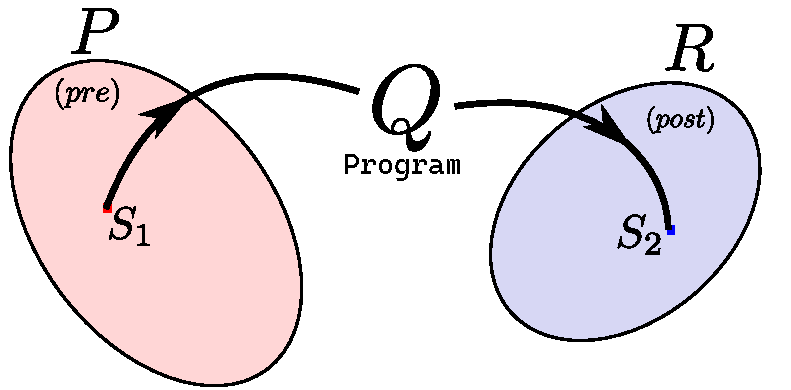
\includegraphics[scale=0.35]{assets/hoare_triple.pdf}
        \end{minipage}
        \hfill
        \pause
        \begin{minipage}{0.5\columnwidth}
            \begin{minted}{c}
                int |$\prog$|(int n){
                    // |$PRE:$ \colorbox{yellow!20!white}{assume(n > 1);}|
                    int i = 0, x = 0;
                    while(i < n){
                        i = i + 1;
                        x = |\boxed{\cdot}|
                    }
                    // |$POST:$ \colorbox{green!10!white}{assert(x > 2 * n);}|
                    return x;
                }
            \end{minted}
        \end{minipage}

    \end{figure}
\end{frame}

\begin{frame}{Lifting Program Sketching to Relational Sketching}

    Given partial programs $\proghole{1}{\cdot}$ and $\proghole{2}{\cdot}$, find completion $\E$, where $\E.H$ and $\E.G$ respective completions of $\proghole{1}{\cdot}$ and $\proghole{2}{\cdot}$ that satisfy a specification.
    \pause
    \vspace{20pt}
    \begin{tcolorbox}[
        colback=white,
        colframe=green,
        colbacktitle=white!70!green,
        coltitle=black,
        title=\textbf{Relational Synthesis},
        enhanced,
        attach boxed title to top left={yshift=-2mm, xshift=0.5cm},%
        ]
        \[ \exists \E. \ \colorbox{yellow!20!white}{\{\textsc{Pre}($\vec{x_1}$, $\vec{x_2}$)\}}\ \proghole{1}{\E.H}, \proghole{2}{\E.G}\ \colorbox{green!20!white}{\{\textsc{Post}($y_1$, $y_2$)\}}
        \]
    \end{tcolorbox}
\end{frame}
\begin{frame}{Verification for Program Equivalence.}
    Program equivalence requires that, any two executions of a pair of programs, $\prog_1$ and $\prog_2$ on same the same input $\vec{x}$, must yield the same outputs.
    \pause
    \begin{tcolorbox}[
        colback=white,
        colframe=green,
        colbacktitle=white!70!green,
        coltitle=black,
        title=\textbf{A Verification Problem},
        enhanced,
        attach boxed title to top left={yshift=-2mm, xshift=0.5cm},%
        ]
        \[
        \forall \vec{x}.\ \prog_1(\vec{x}) = \prog_2(\vec{x})
        \]
    \end{tcolorbox}
    %\pause
    %\begin{tcolorbox}[
    %    colback=white,
    %    colframe=red,
    %    colbacktitle=white!70!red,
    %    coltitle=black,
    %    title=\textbf{Harder Problem!},
    %    enhanced,
    %    attach boxed title to top left={yshift=-2mm, xshift=0.5cm},%
    %]
    %    \[Finding \prog_1\ or\ \prog_2\ may\ only\ be\ \textit{partially specified}.\ \]
    %\end{tcolorbox}
\end{frame}

\begin{frame}{Sketching for Program Equivalence.}
    Given a reference program $\prog_1$ and a \textit{partial} program $\prog_2$ that has a hole $\boxed{\cdot}$, we are interested in \textit{completing} the partial program by synthesizing an expression to fill the hole such that the two programs are rendered semantically equivalent.
    \pause
    \begin{tcolorbox}[
        colback=white,
        colframe=blue,
        colbacktitle=white!70!blue,
        coltitle=black,
        title=\textbf{Formal Definition},
        enhanced,
        attach boxed title to top left={yshift=-2mm, xshift=0.5cm},%
        ]
        \[ \exists \E \in \lang.\ \forall \vec{x}.\ \prog_1(\vec{x}) = \proghole{2}{\E}(\vec{x}) \]
    \end{tcolorbox}
\end{frame}

\begin{frame}[fragile]{Sketching for Program Equivalence}
    %    \frametitle{Program Equivalence}
    \begin{figure}[t]
        \begin{subfigure}{0.48\textwidth}
            \begin{minted}{c}
                int |$\prog_1$|(int n){
                    |\colorbox{yellow!20!white}{assume(n > 1);}|
                    int i = 0, ans = 0;
                    while(i < (n - 1)){
                        i = i + 1;
                        ans = ans + (5 * i) + 1;
                    }
                    return ans + 1;
                }
            \end{minted}
            \caption{Program 1 \label{list:p1}}
        \end{subfigure}
        \begin{subfigure}{0.48\textwidth}
            \begin{minted}{c}
                int |$\proghole{2}{.}$|(int n){
                    |\colorbox{yellow!20!white}{assume(n > 1);}|
                    int x = 0, y = 0, z = n;
                    while(z |$\neq$| 0){
                        z = z - 1;
                        x = |\hole{\cdot}|;
                        y = y + 1;
                    }
                    return x + y;
                }
            \end{minted}
            \caption{Program 2 (with hole \hole{\cdot})\label{list:p2}}
        \end{subfigure}
        %        \caption{Two programs $\prog_1$ and $\proghole{2}{.}$ for program equivalence.\label{list:motiv:eq}}
    \end{figure}
    \pause
    \begin{tcolorbox}[
        colback=white,
        colframe=blue,
        colbacktitle=white!70!blue,
        coltitle=black,
        title=\textbf{Post condition for sketching.},
        enhanced,
        attach boxed title to top left={yshift=-2mm, xshift=0.5cm},%
        ]
        \[ \exists \E \in \lang.\ \forall \vec{x}.\ \prog_1(\vec{x}) = \proghole{2}{\E}(\vec{x}) \]
        \pause
        \vspace{-10pt}
        \[
        \colorbox{green!20!white}{$assert(ans + 1 = x + y)$}
        \]
    \end{tcolorbox}
\end{frame}

\begin{frame}[fragile]{Sketching for Program Equivalence}
    %    \frametitle{Program Equivalence}
    \begin{figure}[t]
        \begin{subfigure}{0.48\textwidth}
            \begin{minted}{c}
                int |$\prog_1$|(int n){
                    |\colorbox{yellow!20!white}{assume(n > 1);}|
                    int i = 0, ans = 0;
                    while(i < (n - 1)){
                        i = i + 1;
                        ans = ans + (5 * i) + 1;
                    }
                    return ans + 1;
                }
            \end{minted}
            \caption{Program 1 \label{list:p1}}
        \end{subfigure}
        \begin{subfigure}{0.48\textwidth}
            \begin{minted}{c}
                int |$\proghole{2}{.}$|(int n){
                    |\colorbox{yellow!20!white}{assume(n > 1);}|
                    int x = 0, y = 0, z = n;
                    while(z |$\neq$| 0){
                        z = z - 1;
                        x = |\hole{x + 6 \cdot y - n}|;
                        y = y + 1;
                    }
                    return x + y;
                }
            \end{minted}
            \caption{Program 2 (with completion)\label{list:p2}}
        \end{subfigure}
        %        \caption{Two programs $\prog_1$ and $\proghole{2}{.}$ for program equivalence.\label{list:motiv:eq}}
    \end{figure}
\end{frame}

\begin{frame}{Strict Equivalence}

    Program equivalence posed as a \textbf{relational} property.
    \pause
    \vspace{20pt}
    \begin{tcolorbox}[
        colback=white,
        colframe=green,
        colbacktitle=white!70!green,
        coltitle=black,
        title=\textbf{Relational Synthesis for Program Equivalence},
        enhanced,
        attach boxed title to top left={yshift=-2mm, xshift=0.5cm},%
        ]
        \[
        \exists \E. \ \{\vec{x_1} = \vec{x_2}\}\ \ \proghole{1}{\E.H}, \proghole{2}{\E.G} \ \colorbox{white}{\{\proghole{1}{\E.H}($\vec{x_1}$) = \proghole{2}{\E.G}($\vec{x_2}$)\}}
        \]
    \end{tcolorbox}

\end{frame}


\begin{frame}{Strict Non-Interference}
    Given public inputs, ($\vec{x_1}, \vec{x_2}$) and secret inputs ($s_1, s_2$), program (\prog) does not reveal any information about the secret inputs.
    \begin{align*}
        \exists \E. \ \{\vec{x_1} = \vec{x_2}\} \ \proghole{}{\E} \ \colorbox{white}{$\{ \proghole{}{\E}({s_1}, \vec{x_1}) = \proghole{}{\E}({s_2}, \vec{x_2}) \}$}
    \end{align*}
\end{frame}

\begin{frame}{Weaker Versions}
    \begin{tcolorbox}[
        colback=white,
        colframe=green,
        colbacktitle=white!70!green,
        coltitle=black,
        title=\textbf{Weak Equivalence},
        enhanced,
        attach boxed title to top left={yshift=-2mm, xshift=0.5cm},%
        ]
        \[
        \exists \E. \ \{\vec{x_1} = \vec{x_2}\}\ \ \proghole{1}{\E.H}, \proghole{2}{\E.G} \colorbox{white}{$\{|| \proghole{1}{\E.H}(\vec{x_1}) - \proghole{2}{\E.G}(\vec{x_2}) || \leq c\}$}
        \]
    \end{tcolorbox}
    \begin{tcolorbox}[
        colback=white,
        colframe=green,
        colbacktitle=white!70!green,
        coltitle=black,
        title=\textbf{Weak Non-Interference},
        enhanced,
        attach boxed title to top left={yshift=-2mm, xshift=0.5cm},%
        ]
        \[
        \exists \E. \ \{\vec{x_1} = \vec{x_2}\} \ \proghole{}{\E} \ \colorbox{white}{$\{||\proghole{}{\E}({s_1}, \vec{x_1}) - \proghole{}{\E}({s_2}, \vec{x_2}) || \leq c\} $}
        \]
    \end{tcolorbox}
\end{frame}

\begin{frame}{Robustness}
    Robustness requires that small changes in the inputs must not lead to large difference in the responses of the program.
    \begin{align*}
        \exists \E. \ \{|| \vec{x_1} - \vec{x_2} || \leq d_1\} \ \proghole{}{\E} \ \colorbox{white}{$\{|| \proghole{}{\E}(\vec{x_1}) - \proghole{}{\E}(\vec{x_2}) || \leq f(\vec{x_1},\vec{x_2})\} $}
    \end{align*}
\end{frame}

\begin{frame}{Group Fairness}
    Program must not use the \textit{sensitive attribute} ($s$) to be unfair to the minority population.
    \begin{align*}
        \exists \E. \ \{{s_1} \leq {s_2} \land \vec{x_2} \sqsubseteq \vec{x_1}\} \ \proghole{}{\E} \ & \colorbox{white}{$\{\proghole{}{\E}(\vec{x_2}, {s_2}) \leq \proghole{}{\E}(\vec{x_1}, {s_1})\} $}
    \end{align*}
\end{frame}

\begin{frame}{Monotonicity}
    Monotonicity is a hyper-property that requires that for any two executions of the program, if the inputs are ordered, so must be the outputs.
    \begin{align*}
        \exists \E. \ \{\vec{x_1} \sqsubseteq \vec{x_2}\} \ \proghole{}{\E}\ \colorbox{white}{$\{ \proghole{}{\E}(\vec{x_1}) \sqsubseteq \proghole{}{\E}(\vec{x_2}) \}$}
    \end{align*}
\end{frame}
\begin{frame}{Relational property with (semantic) quantitative objectives.}
    Quantitative objectives on the synthesis problem that defines the \textit{preference} among the feasible completions, \E.
    \pause
    \vspace{20pt}
    \begin{tcolorbox}[
    colback=white,
    colframe=green,
    colbacktitle=white!70!green,
    coltitle=black,
    title=\textbf{Quantitative Objective, $\Gamma$},
    enhanced,
    attach boxed title to top left={yshift=-2mm, xshift=0.5cm},%
]
    \[
        \Gamma(\ \proghole{1}{\E.H}(\vec{x_1}),\ \proghole{2}{\E.H}(\vec{x_2})\ )
    \]
\end{tcolorbox}
\pause
\vspace{10pt}
The most preferred completion can be found by \textbf{minimizing} the quantitative objective.
\end{frame}

\begin{frame}{Relational property with (semantic) quantitative objectives.}
    The ordering relation $\E$ is a partial order over the completions, defined by the relation, $\sqsubseteq$, and the \textit{strict} ordering $\sqsubset$
    \pause
    \vspace{10pt}
        \begin{tcolorbox}[
        colback=white,
        colframe=green,
        colbacktitle=white!70!green,
        coltitle=black,
        title=\textbf{Dominance},
        enhanced,
        attach boxed title to top left={yshift=-2mm, xshift=0.5cm},%
        ]
A completion $\E'$ dominates a completion $\E$ if the value of $\Gamma$ score with $\E'$ is smaller or equals to $\E$ across all input pairs $\B{\vec{x_1}, \vec{x_2}}$
    \end{tcolorbox}
        \pause
    \vspace{10pt}
    \begin{tcolorbox}[
        colback=white,
        colframe=red,
        colbacktitle=white!70!red,
        coltitle=black,
        title=\textbf{Strict Dominance},
        enhanced,
        attach boxed title to top left={yshift=-2mm, xshift=0.5cm},%
        ]
Additionally requires the existence of at least one input-pair where the $\Gamma$ score of $\E'$ is strictly smaller than that of~$\E$
    \end{tcolorbox}
\end{frame}

\begin{frame}{Objective Function for different Relational Properties.}
    \vspace{20pt}
    \begin{tcolorbox}[
        colback=white,
        colframe=blue,
        colbacktitle=white!70!blue,
        coltitle=black,
        title=\textbf{Monotonicity, Robustness, Weak Non-Interference, Weak Equivalence},
        enhanced,
        attach boxed title to top left={yshift=-2mm, xshift=0.2cm},%
        ]
    Completions that minimize the distance between any two responses of the program.
    \begin{align*}
    \Gamma(\proghole{}{\E}(\vec{x_1}), \proghole{}{\E}(\vec{x_2})) \dfn ||\proghole{}{\E}(\vec{x_1}) - \proghole{}{\E}(\vec{x_2})||
\end{align*}
    \end{tcolorbox}
    \pause
        \vspace{20pt}
    \begin{tcolorbox}[
        colback=white,
        colframe=blue,
        colbacktitle=white!70!blue,
        coltitle=black,
        title=\textbf{Group Fairness},
        enhanced,
        attach boxed title to top left={yshift=-2mm, xshift=0.2cm},%
        ]
        Prefer completions where the deviation in responses between candidates of two populations is small for similar candidates.
    \begin{align*}
        \Gamma(\proghole{}{\E}(\vec{x_1}, {s_1}), \proghole{}{\E}(\vec{x_2}, {s_2})) \dfn \textrm{if } (s_1 < s_2 \land \vec{x_1} \sim \vec{x_2})\\ \textrm{ then }||\proghole{}{\E}(\vec{x_1}, {y_1}) - \proghole{}{\E}(\vec{x_2}, {y_2})|| \textrm{ else } 0
    \end{align*}
    \end{tcolorbox}
\end{frame}

\begin{frame}[fragile]{Monotonicity Example}
    \begin{figure}[t]
        \begin{minted}{c}
            // |PRE: \colorbox{yellow!20!white}{$(a_2 < a_1 \land b_2 > b_1)$}|
            int |$\proghole{}{.}$| (int |$a$|, int |$b$|){
                assume((0 < |$a$|) && (|$a$| < |$b$|));
                while (|$a$| < |$b$|) {
                    |$c$| = |$c$| + |\hole{\cdot}|;
                    |$a$| = |$a$| + 1;
                }
                return |$c$|;
            }
            // |POST: \colorbox{green!20!white}{$(c_2 > c_1)$}|
        \end{minted}
        %\caption{Program Sketch for Monotonicity}
        \label{list:prog:qbsynth}
    \end{figure}
\end{frame}

\begin{frame}[fragile]{Monotonicity Example: Product Program}
    \centering
    \begin{figure}[t]
        \begin{minted}{java}
            int |$\widehat{\proghole{}{\cdot}}$|(int |$a_1$|, int |$b_1$|, int |$a_2$|, int |$b_2$|){

                assume((0 < |$a_1$|) && (|$a_1$| < |$b_1$|));
                assume((0 < |$a_2$|) && (|$a_2$| < |$b_2$|));
                assume((|$a_2$| < |$a_1$|) && (|$b_2$| > |$b_1$|));

                int |$c_1$| = 0, |$c_2$| = 0;
                while (|\colorbox{yellow}{$(a_1 < b_1)$}| |$\mid\mid$| |\colorbox{green!40!white}{$(a_2 < b_2)$}|) {
                    if (|\colorbox{yellow}{$(a_1 < b_1)$}|) {
                        |$c_1$| = |$c_1$| + |\hole{\cdot}|;
                        |$a_1$| = |$a_1$| + 1;
                    }
                    if (|\colorbox{green!40!white}{$(a_2 < b_2)$}|) {
                        |$c_2$| = |$c_2$| + |\hole{\cdot}|;
                        |$a_1$| = |$a_1$| + 1;
                    }
                }
                return |$c_1,\ c_2$|;
            }
        \end{minted}
        %\caption{Product program for Monotonicity from \Cref{list:prog:qbsynth}.}
        %label{list:pp:qbsynth}
    \end{figure}
\end{frame}

\begin{frame}{Tool Architecture}
    \begin{figure}
        \centering
        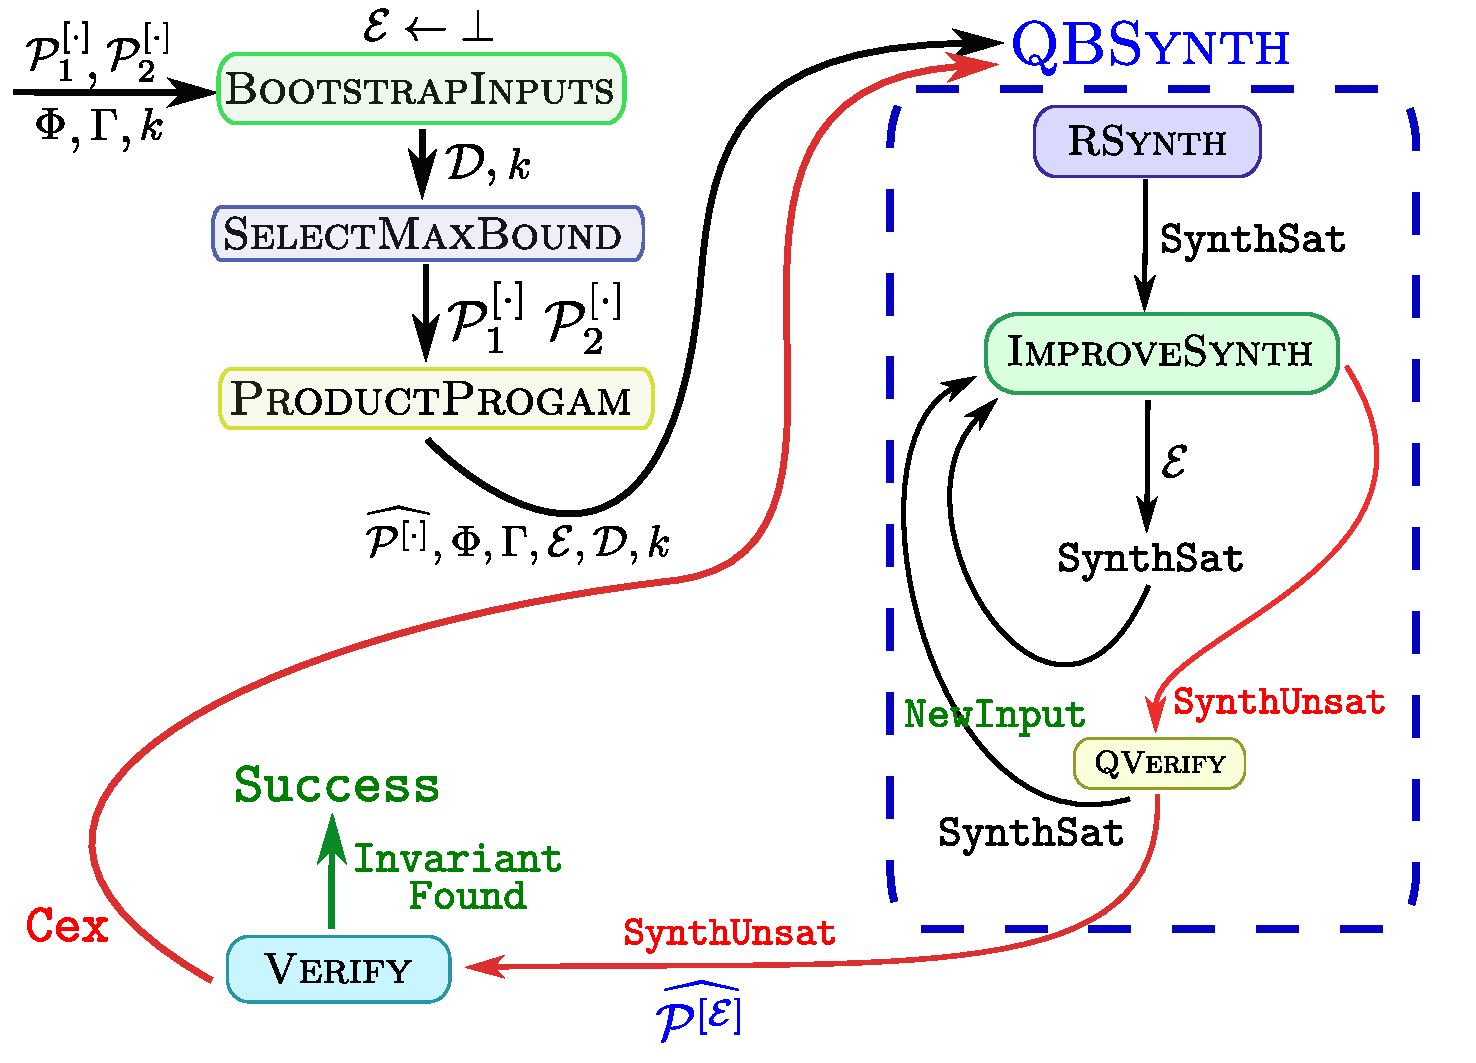
\includegraphics[scale=0.45]{assets/tool_arch.pdf}
    \end{figure}
\end{frame}

\begin{frame}[fragile]{Monotonicity Example: Product Program}
    \centering
    \begin{figure}[t]
        \begin{minted}{java}
            int |$\widehat{\proghole{}{\cdot}}$|(int |$a_1$|, int |$b_1$|, int |$a_2$|, int |$b_2$|){

                assume((0 < |$a_1$|) && (|$a_1$| < |$b_1$|));
                assume((0 < |$a_2$|) && (|$a_2$| < |$b_2$|));
                assume((|$a_2$| < |$a_1$|) && (|$b_2$| > |$b_1$|));

                int |$c_1$| = 0, |$c_2$| = 0;
                while (|\colorbox{yellow}{$(a_1 < b_1)$}| |$\mid\mid$| |\colorbox{green!40!white}{$(a_2 < b_2)$}|) {
                    if (|\colorbox{yellow}{$(a_1 < b_1)$}|) {
                        |$c_1$| = |$c_1$| + |\hole{\cdot}|;
                        |$a_1$| = |$a_1$| + 1;
                    }
                    if (|\colorbox{green!40!white}{$(a_2 < b_2)$}|) {
                        |$c_2$| = |$c_2$| + |\hole{\cdot}|;
                        |$a_1$| = |$a_1$| + 1;
                    }
                }
                return |$c_1,\ c_2$|;
            }
        \end{minted}
        %\caption{Product program for Monotonicity from \Cref{list:prog:qbsynth}.}
        %label{list:pp:qbsynth}
    \end{figure}
\end{frame}

\begin{frame}[fragile]{Monotonicity Example: First Completion}
        \begin{figure}[t]
        \begin{minipage}{0.45\columnwidth}
        \begin{minted}{c}
            // |PRE: \colorbox{yellow!20!white}{$(a_2 < a_1 \land b_2 > b_1)$}|
            int |$\proghole{}{.}$| (int |$a$|, int |$b$|){
                assume((0 < |$a$|) && (|$a$| < |$b$|));
                while (|$a$| < |$b$|) {
                    |$c$| = |$c$| + |\hole{b}|;
                    |$a$| = |$a$| + 1;
                }
                return |$c$|;
            }
            // |POST: \colorbox{green!20!white}{$(c_2 > c_1)$}|
        \end{minted}
        \end{minipage}
        \begin{minipage}{0.45\columnwidth}
            \centering
            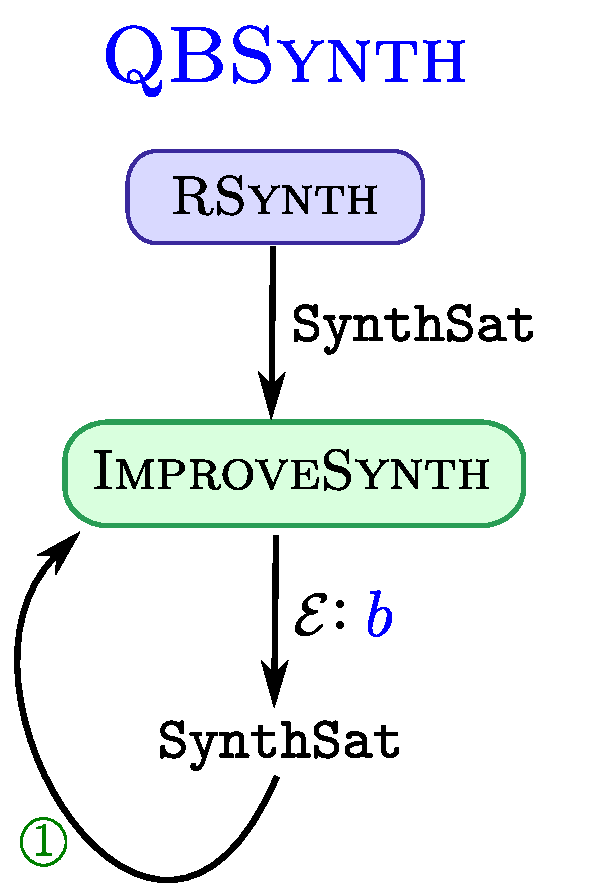
\includegraphics[scale=0.3]{assets/stage1.pdf}
        \end{minipage}
    \end{figure}
\end{frame}

\begin{frame}[fragile]{Monotonicity Example: Second Completion}
        \begin{figure}[t]
    \begin{minipage}{0.45\columnwidth}
        \begin{minted}{c}
            // |PRE: \colorbox{yellow!20!white}{$(a_2 < a_1 \land b_2 > b_1)$}|
            int |$\proghole{}{.}$| (int |$a$|, int |$b$|){
                assume((0 < |$a$|) && (|$a$| < |$b$|));
                while (|$a$| < |$b$|) {
                    |$c$| = |$c$| + |\hole{1}|;
                    |$a$| = |$a$| + 1;
                }
                return |$c$|;
            }
            // |POST: \colorbox{green!20!white}{$(c_2 > c_1)$}|
        \end{minted}
    \end{minipage}
    \begin{minipage}{0.45\columnwidth}
        \centering
        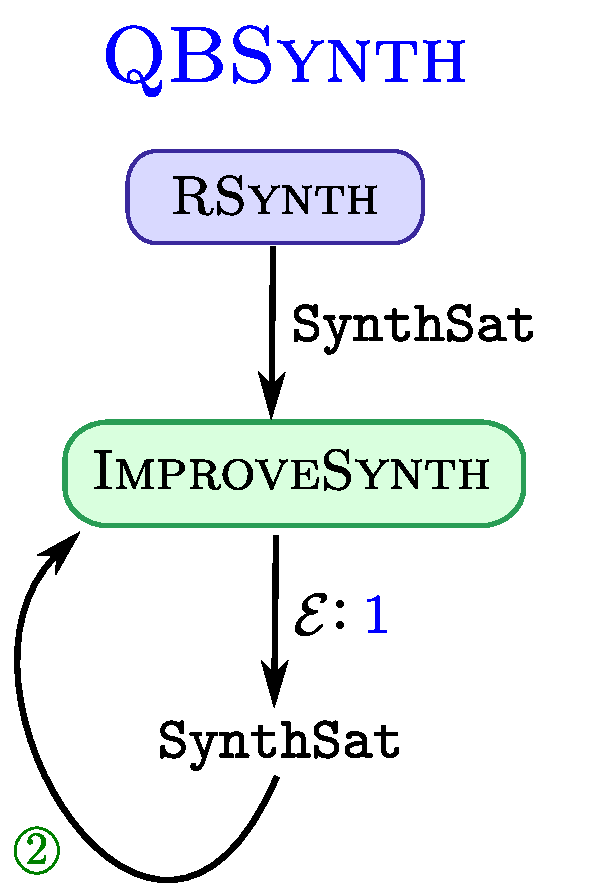
\includegraphics[scale=0.3]{assets/stage2.pdf}
    \end{minipage}
\end{figure}
\end{frame}

\begin{frame}[fragile]{Monotonicity Example: Third Completion}
        \begin{figure}[t]
    \begin{minipage}{0.45\columnwidth}
        \begin{minted}{c}
            // |PRE: \colorbox{yellow!20!white}{$(a_2 < a_1 \land b_2 > b_1)$}|
            int |$\proghole{}{.}$| (int |$a$|, int |$b$|){
                assume((0 < |$a$|) && (|$a$| < |$b$|));
                while (|$a$| < |$b$|) {
                    |$c$| = |$c$| + |\hole{(b - c) + 1}|;
                    |$a$| = |$a$| + 1;
                }
                return |$c$|;
            }
            // |POST: \colorbox{green!20!white}{$(c_2 > c_1)$}|
        \end{minted}
    \end{minipage}
    \begin{minipage}{0.45\columnwidth}
        \centering
        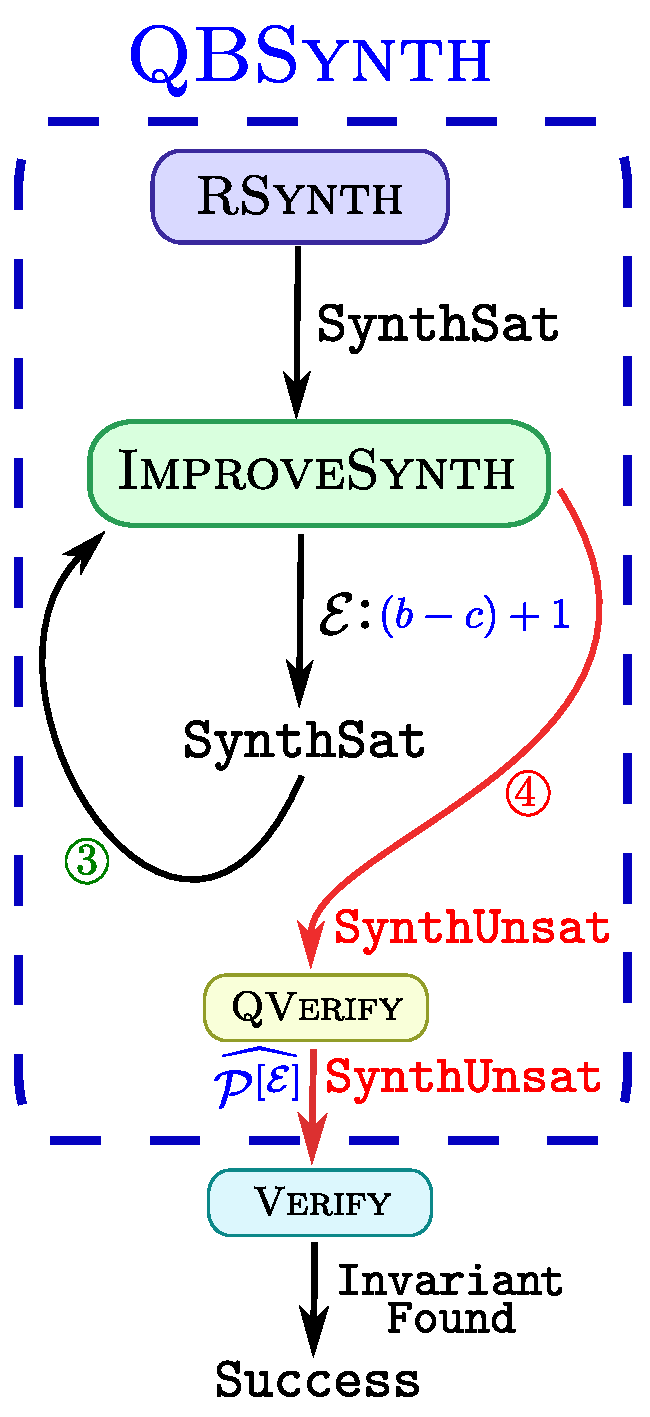
\includegraphics[scale=0.3]{assets/stage3.pdf}
    \end{minipage}
\end{figure}
\end{frame}

\begin{frame}{Experiments}
    Machine configuration, Benchmark Sources, Domain-specific Language.
\end{frame}

\begin{frame}{Instances without quantitative objectives.}
    \begin{table}
        \centering
        \small
        %\captionof{table}{Instances without quantitative objectives.}
        \label{tab:rsynth}
        \begin{tabular}{c|c|c}
            \toprule
            \textbf{Bench} & \textbf{Property} & \textbf{Time(s)} \\ \hline\hline
            b26 & {\textbf{\begin{tabular}[c]{@{}c@{}}Strict Equivalence\end{tabular}}} & 4 \\ \hline
            b10 & {\textbf{\begin{tabular}[c]{@{}c@{}}Strict Equivalence\end{tabular}}} & 3 \\ \hline
            b18 & {\textbf{\begin{tabular}[c]{@{}c@{}}Strict Equivalence\end{tabular}}} & 2 \\ \hline
            b16 & {\textbf{\begin{tabular}[c]{@{}c@{}}Strict Equivalence\end{tabular}}} & 1 \\ \hline
            b21 & {\textbf{\begin{tabular}[c]{@{}c@{}}Strict Equivalence\end{tabular}}} & 3 \\ \hline
            b27 & {\textbf{\begin{tabular}[c]{@{}c@{}}Strict Equivalence\end{tabular}}} & 4 \\ \hline
            b04 & {\textbf{\begin{tabular}[c]{@{}c@{}}Strict Equivalence\end{tabular}}} & 3 \\ \hline
            b34 & {\textbf{\begin{tabular}[c]{@{}c@{}}Strict Equivalence\end{tabular}}} & 10 \\ \hline
            b05 & {\textbf{\begin{tabular}[c]{@{}c@{}}Strict Equivalence\end{tabular}}} & 7 \\ \hline
            nonintf01 & {\textbf{\begin{tabular}[c]{@{}c@{}}Strict Non-Interference\end{tabular}}} & 7 \\ \hline
            nonintf02 & {\textbf{\begin{tabular}[c]{@{}c@{}}Strict Non-Interference\end{tabular}}} & 8 \\ \hline
            nonintf05 & {\textbf{\begin{tabular}[c]{@{}c@{}}Strict Non-Interference\end{tabular}}} & 6 \\ \hline
        \end{tabular}
    \end{table}
\end{frame}

\begin{frame}{Instances with quantitative objectives}
    \begin{table}
        \centering
        \small
        %\captionof{table}{Instances with quantitative objectives}
        \label{tab:qbsynth}
        \begin{tabular}{c|c|c|c}
            \toprule
            \textbf{Bench} & \textbf{Property} & \textbf{Time(s)} & \textbf{Best?} \\ \hline\hline
            mono01 & {\textbf{\begin{tabular}[c]{@{}c@{}}Monotonicity\end{tabular}}} & 329 & \textcolor{green}{\ding{52}} \\ \hline
            mono02 & {\textbf{\begin{tabular}[c]{@{}c@{}}Monotonicity\end{tabular}}} & 311 & \textcolor{green}{\ding{52}} \\ \hline
            mono02 & {\textbf{\begin{tabular}[c]{@{}c@{}}Monotonicity\end{tabular}}} & 310 & \textcolor{green}{\ding{52}} \\ \hline
            weak01 & {\textbf{\begin{tabular}[c]{@{}c@{}}Weak Equivalence\end{tabular}}} & 210 & \textcolor{green}{\ding{52}} \\ \hline
            weak02 & {\textbf{\begin{tabular}[c]{@{}c@{}}Weak Equivalence\end{tabular}}} & 198 & \textcolor{green}{\ding{52}} \\ \hline
            weak03 & {\textbf{\begin{tabular}[c]{@{}c@{}}Weak Equivalence\end{tabular}}} & 128 & \textcolor{green}{\ding{52}} \\ \hline
            weak04 & {\textbf{\begin{tabular}[c]{@{}c@{}}Weak Equivalence\end{tabular}}} & 168 & \textcolor{green}{\ding{52}} \\ \hline
            robust01 & {\textbf{\begin{tabular}[c]{@{}c@{}}Robustness\end{tabular}}} & 95 & \textcolor{green}{\ding{52}} \\ \hline
            robust02 & {\textbf{\begin{tabular}[c]{@{}c@{}}Robustness\end{tabular}}} & 102 & \textcolor{green}{\ding{52}} \\ \hline
            fair01 & {\textbf{\begin{tabular}[c]{@{}c@{}}Group Fairness\end{tabular}}} & 82 & \textcolor{green}{\ding{52}} \\ \hline
            nonintf03 & {\textbf{\begin{tabular}[c]{@{}c@{}}Weak Non-Interference\end{tabular}}} & 70 & \textcolor{green}{\ding{52}} \\ \hline
            nonintf04 & {\textbf{\begin{tabular}[c]{@{}c@{}}Weak Non-Interference\end{tabular}}} & 75 & \textcolor{green}{\ding{52}} \\ \hline
        \end{tabular}
    \end{table}
\end{frame}

\begin{frame}{Conclusion \& Future Directions}
    \vspace{10pt}
    \begin{tcolorbox}[
        colback=white,
        colframe=green,
        colbacktitle=white!70!green,
        coltitle=black,
        title=\textbf{New Synthesis Problem!},
        enhanced,
        attach boxed title to top left={yshift=-2mm, xshift=0.2cm},%
        ]
          Relational synthesis with semantic quantitative objectives---and designed an algorithm to solve the same.
    \end{tcolorbox}
    \pause
    \vspace{5pt}
    \begin{tcolorbox}[
        colback=white,
        colframe=blue,
        colbacktitle=white!70!blue,
        coltitle=black,
        title=\textbf{Conclusion},
        enhanced,
        attach boxed title to top left={yshift=-2mm, xshift=0.2cm},%
        ]
   \begin{itemize}
    \item[-] \tool instantiates this algorithm and solves non-trivial problems in a reasonable time.
    \item[-] Our solutions are optimal only for a $k$-bounded setting, however, we do achieve the globally optimal completions (empirically) for all benchmarks in our suite.
\end{itemize}
    \end{tcolorbox}
   \pause
   \vspace{5pt}
       \begin{tcolorbox}[
       colback=white,
       colframe=yellow!20!black,
       colbacktitle=white!70!yellow,
       coltitle=black,
       title=\textbf{Future Directions},
       enhanced,
       attach boxed title to top left={yshift=-2mm, xshift=0.2cm},%
       ]
   \begin{itemize}
    \item[-] Synthesis for global optimality.
    \item[-] Synthesis problems for those beyond 2-safety.
\end{itemize}
   \end{tcolorbox}
\end{frame}

\begin{frame}{Thank You!}
   \huge{Questions?}
\end{frame}

\end{document}